\documentclass{article}

% if you need to pass options to natbib, use, e.g.:
%     \PassOptionsToPackage{numbers, compress}{natbib}
% before loading neurips_2020

% ready for submission
 \usepackage{neurips_2020}

% to compile a preprint version, e.g., for submission to arXiv, add add the
% [preprint] option:
%     \usepackage[preprint]{neurips_2020}

% to compile a camera-ready version, add the [final] option, e.g.:
%     \usepackage[final]{neurips_2020}

% to avoid loading the natbib package, add option nonatbib:
%     \usepackage[nonatbib]{neurips_2020}

\usepackage[utf8]{inputenc} % allow utf-8 input
\usepackage[T1]{fontenc}    % use 8-bit T1 fonts
\usepackage{hyperref}       % hyperlinks
\usepackage{url}            % simple URL typesetting
\usepackage{booktabs}       % professional-quality tables
\usepackage{amsfonts}       % blackboard math symbols
\usepackage{nicefrac}       % compact symbols for 1/2, etc.
\usepackage{microtype}      % microtypography

\usepackage{amsmath}
\usepackage{graphicx}
\usepackage{enumerate}
\usepackage{natbib}
\usepackage{url}
\usepackage{enumitem}

\usepackage{amsmath,amssymb,amsthm,bm,mathtools}
\usepackage{algorithm}
\usepackage{dsfont,multirow,hyperref,setspace,enumerate}
\hypersetup{colorlinks,linkcolor={black},citecolor={black},urlcolor={black}}

\theoremstyle{definition}
\newtheorem{thm}{Theorem}[section]
\newtheorem{lem}{Lemma}
\newtheorem{prop}{Proposition}
\newtheorem{pro}{Property}
\newtheorem{cor}{Corollary}[section]

\theoremstyle{definition}
\newtheorem{assumption}{Assumption}
\newtheorem{defn}{Definition}
\newtheorem{example}{Example}
\newtheorem{rmk}{Remark}

\usepackage{appendix}
\usepackage{wrapfig}
\mathtoolsset{showonlyrefs}


\usepackage{algpseudocode,algorithm}
\algnewcommand\algorithmicinput{\textbf{Input:}}
\algnewcommand\algorithmicoutput{\textbf{Output:}}
\algnewcommand\INPUT{\item[\algorithmicinput]}
\algnewcommand\OUTPUT{\item[\algorithmicoutput]}




\usepackage{xr}

\input macros.tex


\title{Learning Multiple Networks via Supervised Tensor Decomposition}

% The \author macro works with any number of authors. There are two commands
% used to separate the names and addresses of multiple authors: \And and \AND.
%
% Using \And between authors leaves it to LaTeX to determine where to break the
% lines. Using \AND forces a line break at that point. So, if LaTeX puts 3 of 4
% authors names on the first line, and the last on the second line, try using
% \AND instead of \And before the third author name.

%\author{%}

\begin{document}

\maketitle

\begin{abstract}
   We develop a tensor decomposition method that incorporates multiple side information as interactive features. Unlike unsupervised tensor decomposition, our supervised decomposition captures the effective dimension reduction of the data tensor confined to feature space on each mode. An efficient alternating optimization algorithm is further developed. Our proposal handles a broad range of data types, including continuous, count, and binary observations. We apply the method to diffusion tensor imaging data from human connectome project. We identify the key global brain connectivity pattern and pinpoint the local regions that are associated with available features. Our method will help the practitioners efficiently analyze tensor datasets in various areas.
\end{abstract}

\section{Introduction}
 Higher-order tensors have received increased attention across science and engineering. While most tensor decomposition methods are developed for a single tensor observation, scientific studies often collect side information, in the form of node features and interactions thereof, together with the tensor data. Such data problems are common in neuroimaging, network analysis, and spatial-temporal modeling. A popular example is in neuroimaging~\citep{zhou2013tensor}. The brain connectivity networks are collected from a sample of individuals, accompanied by individual characteristics such as age, gender, and diseases status (see Figure~\ref{fig:intro1}a). Another example is in network analysis~\citep{pmlr-v108-berthet20a,hoff2005bilinear}. A typical social network consists of nodes that represent people and edges that represent  friendships. Side information such as people’s demographic information and friendship types are often available. In both examples, it is of keen scientific interest to identify the variation in the data tensor (e.g., brain connectivities, social community patterns) that is affected by available features. These seemingly different scenarios pose a common yet challenging problem for tensor data modeling. 
 
 \begin{figure}[hbt]
\begin{center}
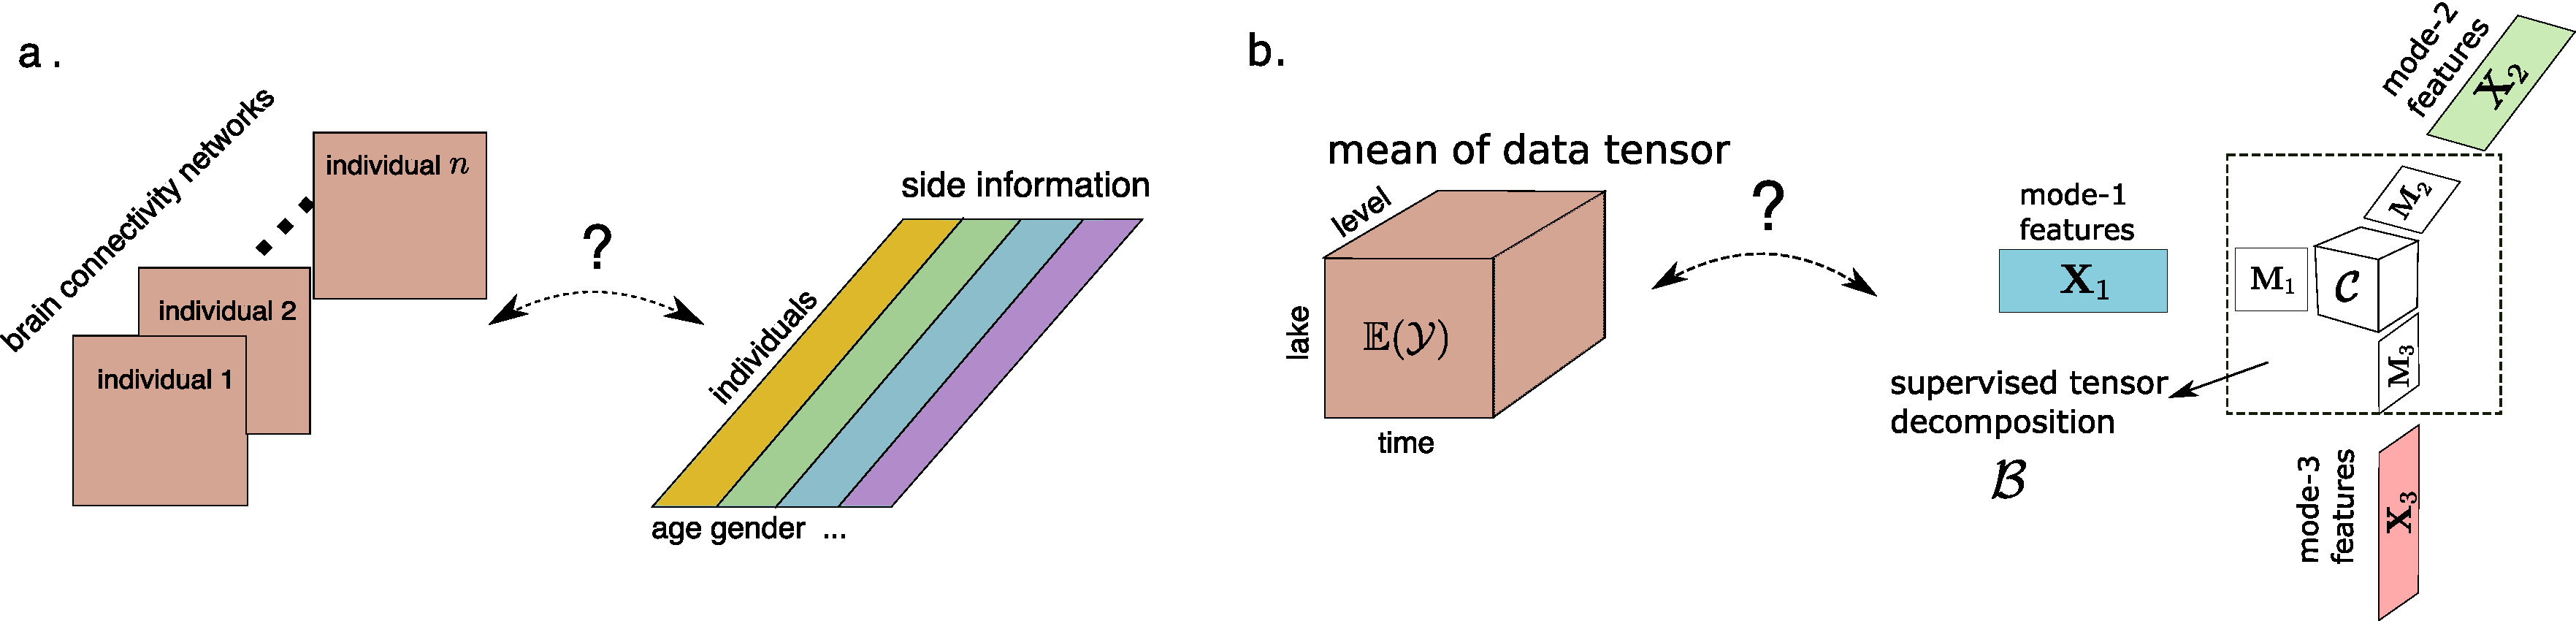
\includegraphics[width = 13.5cm]{demo.pdf}
\vspace{-.5cm}
\end{center}
\caption{Examples of supervised tensor decomposition with interactive side information. (a) Network population model. (b) Spatio-temporal growth model.} \label{fig:intro1}
\vspace{-.3cm}
\end{figure}

In addition to the aforementioned challenges, many tensor datasets consist of non-Gaussian measurements. Classical tensor decomposition methods are based on minimizing the Frobenius norm of deviation, leading to suboptimal predictions for binary- or count-valued response variables. A number of supervised tensor methods have been proposed \citep{narita2012tensor, zhao2012higher, yu2016learning,lock2018supervised}. These methods often assume Gaussian distribution for the tensor entries, or impose random designs for the feature matrices, both of which are less suitable for applications of our interest. The gap between theory and practice means a great opportunity to modeling paradigms and better capture the complexity in tensor data. 

We present a general model and associated method for decomposing a data tensor whose entries are from exponential family with interactive side information. We formulate the learning task as a structured regression problem, with tensor observation serving as the response, and the multiple side information as interactive features. We leverage generalized linear model (GLM)  to allow heteroscedacity due to the mean-variance relationship in the non-Gaussian data. The low-rank structure on the conditional mean tensor effectively mitigates the curse of high dimensionality.  Our proposal blends the modeling power of GLM and the exploratory capability of tensor dimension reduction in order to take the best out of both worlds. 
%A low-rank structure is imposed to the conditional mean of tensor observation.where unlike classical decomposition, the tensor factors $\mX_k\mM_k\in\mathbb{R}^{d_k\times r_k}$ belong to the space spanned by features $\mX_k\in\mathbb{R}^{d_k\times p_k}$ for $k=1,2,3$. The unknown matrices $\mM_k\in\mathbb{R}^{p_k\times r_k}$ (referred to as ``dimension reduction matrices'') link the conditional mean to the feature spaces, thereby allowing the identification of variations in the tensor data attributable to the side information.


 % This flexibility is important in practice. Furthermore, our low-rank model on the (transformed) conditional mean tensor effectively mitigates the curse of high dimensionality. In classical GLM, the sample size and feature dimension are well defined; however, in the tensor data analysis, we observe only one realization of an order-$K$ tensor and up to $K$ interactive feature matrices. Both the number of tensor entries and feature dimension grow exponentially in $K$. Dimension reduction is therefore crucial for prediction and interpretability. We establish the statistical convergence of our estimator, and we quantify the gain in prediction through simulations and case studies.
  
\vspace{-0.3cm}

\section{Method}

\subsection{Preliminary}
We introduce the basic tensor properties used in the paper. We use lower-case letters (e.g.,\ $a,b,c$) for scalars and vectors, upper-case boldface letters (e.g.,\ $\mA, \mB, \mC$) for matrices, and calligraphy letters (e.g.,\ $\tA, \tB, \tC$) for tensors of order three or greater. Let $\tY=\entry{y_{i_1,\ldots,i_K}}\in \mathbb{R}^{d_1\times \cdots\times d_K}$ denote an order-$K$ $(d_1,\ldots,d_K)$-dimensional tensor. The multilinear multiplication of a tensor $\tY\in\mathbb{R}^{d_1\times \cdots\times d_K}$ by matrices $\mX_k=\entry{x_{i_k,j_k}^{(k)}}\in\mathbb{R}^{p_k\times d_k}$ is defined as $\tY\times\{\mX_1,\ldots,\mX_K\} =\entry{\sum_{i_1,\ldots,i_K}y_{i_1,\ldots,i_K}x_{j_1,i_1}^{(1)}\cdots x_{j_K,i_K}^{(K)}}$,
which results in an order-$K$ $(p_1,\ldots,p_K)$-dimensional tensor.For any two tensors $\tY=\entry{y_{i_1,\ldots,i_K}}$, $\tY'=\entry{y'_{i_1,\ldots,i_K}}$ of identical order and dimensions, their inner product is defined as $\langle \tY,\ \tY'\rangle =\sum_{i_1,\ldots,i_K}y_{i_1,\ldots,i_K}y'_{i_1,\ldots,i_K}.$
The tensor Frobenius norm is defined as $\FnormSize{}{\tY}=\langle \tY,\ \tY \rangle^{1/2}$, and the maximum norm is defined $\mnormSize{}{\tY}=\max_{i_1,\ldots,i_K}y_{i_1,\ldots,i_K}.$  We let $\mI_d$ denote the $d \times d$ identity matrix and $[d]$ denote the $d$-set $\{1,\ldots,d\}$.
%For any two matrices $\mA,\mB$ with orthonormal columns of same dimension, the angle distance is defined as
%\[ \sin \Theta(\mA,\mB)=\snormSize{}{\mA^T \mB^{\perp}}=\max\left\{ \frac{\langle \mx, \my\rangle}{\vnormSize{}{\mx}\vnormSize{}{\my}}\colon \ \mx\in \textup{Span}(\mA),\ \my\in \textup{Span}(\mB^\perp)\right\}. \]


\subsection{General Model}

Let $\tY=\entry{y_{i_1,\ldots,i_K}}\in\mathbb{R}^{d_1\times \cdots\times d_K}$ denote an order-$K$ data tensor. Suppose the side information is available on each of the $K$ modes. Let $\mX_k=\entry{x_{ij}}\in\mathbb{R}^{d_k\times p_k}$ denote the feature matrix on the mode $k\in[K]$, where $x_{ij}$ denotes the $j$-th feature value for the $i$-th tensor entity, for $(i,j)\in[d_k]\times[p_k]$, $p_k\leq d_k$. Assume that, conditional on the features $\mX_k$, the entries of tensor $\tY$ are independent realizations from an exponential family distribution, and the conditional mean tensor admits the form
\begin{align}\label{eq:tensormodel}
&\mathbb{E}(\tY|\mX_1,\ldots,\mX_K)=f(\Theta),\quad \text{with}\quad \Theta =\tB\times\{\mX_1,\ldots, \mX_K\} ,
\end{align}
where $\Theta\in\mathbb{R}^{d_1\times \cdots\times d_K}$ is the multilinear predictor, $\tB\in\mathbb{R}^{p_1\times \cdots \times p_K}$ is the unknown parameter tensor, $f(\cdot)$ is a known link function whose form depending on the data type of $\tY$. The choice of link function is based on the assumed distribution family of tensor entries. 

In classical tensor decomposition, tensor factorization is performed on either data tensor $\tY$ or mean tensor $\mathbb{E}(\tY)$. In the context of supervised tensor decomposition, we propose to factorize the latent parameter tensor $\tB$,
\begin{equation}\label{eq:factor}
\tB=\tC\times\{\mM_1,\ \ldots,\ \mM_K\},
\end{equation}
where $\tC\in\mathbb{R}^{r_1\times \cdots \times r_K}$ is a full-rank core tensor, and $\mM_k\in\mathbb{R}^{p_k\times r_k}$ are factor matrices consisting of orthonormal columns, where $r_k\leq p_k$ for all $k\in[K]$. By the definition of multilinear rank, model equations~\eqref{eq:tensormodel} and~\eqref{eq:factor} imply the low-rankness $\mr=(r_1,\ldots,r_K)$ of the conditional mean tensor under the link function. We now reach our final model for supervised tensor decomposition,
\begin{align}\label{eq:decomp}
\mathbb{E}(\tY|\mX_1,\ldots,\mX_K) &= f\left(\tC\times\{\mX_1\mM_1, \ldots, \mX_K\mM_K\}\right),\notag\\
\text{with} \ &\ \mM_k^T\mM_k = \mI_{r_k},\ \mM_k\in\mathbb{R}^{p_k\times r_k}\quad \text{for all }k=1,\ldots,K,
\end{align}
where the parameters of interest are $\mM_k$ and $\tC$. Note that model~\eqref{eq:decomp} assumes a fixed, known rank $\mr=(r_1,\ldots,r_K)$. Figure~\ref{fig:intro1}b provides a schematic illustration of our model. The features $\mX_k$ affect the distribution of tensor entries in $\tY$ through the form $\mX_k\mM_k$, which are $r_k$ linear combinations of features on mode $k$. We call $\mX_k\mM_k$ the ``supervised tensor factors'' or ``sufficient features''~\citep{adragni2009sufficient}, and call $\mM_k$ the ``dimension reduction matrix.'' The core tensor $\tC$ collects the interaction effects between sufficient features across $K$ modes, which links the conditional mean to the feature spaces, and thereby allows the identification of variations in the tensor data attributable to the side information. Our goal is to find $\mM_k$ and the corresponding $\tC$. Note that $\mM_k$ and $\tC$ are identifiable only up to orthonormal transformations.  

\vspace{-.3cm}
\section{Estimation}
\subsection{Rank-constrained M-estimator}
 We adopt the exponential family as a flexible framework for different data types. In a classical generalized linear model with a scalar response $y$ and feature $\mx$, the density is expressed as
\[
p(y|\mx, \boldsymbol{\beta})=c(y,\phi)\exp\left(\frac{y\theta- b(\theta)}{\phi}\right)\ \text{with}\ \theta=\boldsymbol{\beta}^T\mx,
\]
where $b(\cdot)$ is a known function depending on the data types, $\theta$ is the linear predictor, $\phi>0$ is the dispersion parameter, and $c(\cdot)$ is a known normalizing function. In our context, we model the tensor entries $y_{i_1,\ldots,i_K}$, conditional on $\theta_{i_1,\ldots,i_K}$, as independent draws from an exponential family. Ignoring constants that do not depend on $\Theta$, the quasi log-likelihood of~\eqref{eq:decomp} is equal to Bregman distance between $\tY$ and $b'(\Theta)$:
\begin{equation}\label{eq:loglikelihood}
\small
\tL_{\tY}(\tC,\mM_1,\ldots,\mM_K)=\langle \tY, \Theta \rangle - \sum\nolimits_{i_1,\ldots,i_K} b(\theta_{i_1,\ldots,i_K})\ \text{with}\ \Theta=\tC\times\{\mM_1\mX_1,\ldots,\mM_K\mX_K\}.
\end{equation}
We propose a constrained maximum quasi-likelihood estimator (M-estimator),
\begin{align} \label{eq:MLE} 
(\hat \tC, \hat \mM_1,\ldots,\hat \mM_k) &=\argmax_{(\tC,\mM_1,\ldots,\mM_K)\in \tP} \ \tL_{\tY}(\tC,\mM_1,\ldots,\mM_K),
\end{align}
where parameter space 
$
\tP=\left\{(\tC, \mM_1,\ldots,\mM_K) \ \Big| \ \mM_k^T\mM_k=\mathbf{I}_{r_k},\ \mnormSize{}{\Theta(\tC,\mM_1,\ldots,\mM_K)}\leq \alpha \right\}.
$
The maximum norm constraint on the linear predictor $\Theta$ is a technical condition to avoid the divergence in the non-Gaussian variance.


\subsection{Alternating optimization}

The decision variables in the objective function~\eqref{eq:MLE} consist of $K+1$ blocks of variables, one for the core tensor $\tC$ and $K$ for the factor matrices $\mM_k$. We notice that, if any $K$ out of the $K+1$ blocks of variables are known, then the optimization reduces to a simple GLM with respect to the last block of variables. This observation leads to an iterative updating scheme for one block at a time while keeping others fixed.  A simplified version of the algorithm is described in Algorithm~\ref{alg:B}. 

\begin{algorithm}[!h]
\caption{Supervised Tensor Decomposition with Interactive Side Information (Simplified)}\label{alg:B}
\begin{algorithmic}[1]
\INPUT Response tensor $\tY\in \mathbb{R}^{d_1\times \cdots \times d_K}$, feature matrices $\mX_k\in\mathbb{R}^{d_k\times p_k}$ for $k=1,\ldots,K$, target Tucker rank $\mr=(r_1,\ldots,r_K)$, link function $f$, maximum norm bound $\alpha$
\OUTPUT Estimated core tensor $\hat \tC\in\mathbb{R}^{r_1\times \cdots \times r_K}$ and factor matrices $\hat \mM_k\in\mathbb{R}^{p_k\times r_k}$. 
\State Random initialization of the core tensor $\tC$ and factor matrices $\mM_k$. 
\While{Do until convergence}

%\State Obtain the factor matrix $\tilde \mM_k\in\mathbb{R}^{p_k\times r_k}$ by a GLM with link function $f$.
%\State Perform QR factorization $\tilde \mM_k=\mQ\mR$.
%\State Update $\mM_k\leftarrow \mQ$ and core tensor $\tC\leftarrow \tC\times_k \mR$.
\State Obtain $\tilde \mM_k\in\mathbb{R}^{p_k\times r_k}$ by a GLM. Orthogonalize $\tilde \mM_k$ by QR factorization, for $k \in [K]$. 

\State Update the core tensor $\tC$ by solving a GLM. Rescale the core tensor $\tC$ such that $\maxnorm{\tC} \leq \alpha$. 
\EndWhile
\end{algorithmic}
\end{algorithm}

\subsection{Statistical properties}\label{subsec:statprob}

In modern applications, the tensor data and features are often large-scale. We are particularly interested in the high-dimensional regime in which both $d_k$ and $p_k$ diverge; i.e.\ $d_k\to \infty$ and $p_k\to\infty$, while $p_k/d_k \to \gamma_k \in[0,1)$. As the size of problem grows, and so does the number of unknown parameters. The classical MLE theory does not directly apply. We leverage the recent development in random tensor theory and high-dimensional statistics to establish the error bounds.

 
\begin{thm}[Statistical convergence]\label{thm:main}
Consider a data tensor generated from model~\eqref{eq:decomp}. Let $(\hat \tC, \hat \mM_1,\ldots,\hat \mM_K)$ be the M-estimator in~\eqref{eq:MLE} and $\hat \tB=\hat \tC\times \hat \mM_1\times\cdots \times \hat \mM_K$. Define $r_\textup{total}=\prod_k r_k$ and $r_{\max}=\max_k r_k$. Under mild technical assumptions, there exist two positive constants $C_1=C_1(\alpha,K), C_2=C_2(\alpha, K)>0$ independent of dimensions $\{d_k\}$ and $\{p_k\}$, such that, with probability at least $1-\exp(-C_1\sum_k p_k)$, 
\begin{equation}\label{eq:bound}
    \FnormSize{}{\trueB- \hat \tB}^2\leq \frac{ C_{2} r_{\textup{total}}}{r_{\max}}\frac{\sum_k p_k}{\prod_k d_k}.
\end{equation}
Furthermore, if the unfolded core tensor has non-degenerate singular values at mode $k\in[K]$, i.e., $\sigma_{\min}(\textup{Unfold}_k(\tC_\textup{true})) \geq c>0$ for some constant $c$, then
\begin{equation}\label{eq:sinebound}
\textup{sin}^2 \Theta(\trueM,\ \hat \mM_k) \leq  \frac{ C_{2}r_{\textup{total}}}{ r_{\max}\sigma^2_{\min}(\textup{Unfold}_k(\tC_\textup{true}))}\frac{\sum_k p_k}{\prod_k d_k},
\end{equation}
where $
\sin \Theta(\trueM,\hat \mM_k)=\snormSize{}{\trueM^T \hat \mM_k^{\perp}}=\max\left\{ \frac{\langle \mx, \my\rangle}{\vnormSize{}{\mx}\vnormSize{}{\my}}\colon \ \mx\in \textup{Span}(\trueM),\ \my\in \textup{Span}({\hat \mM_k}^\perp)\right\}
$ is the angle distance to assess the accuracy in estimating the column space, $\textup{Span}(\mM_k)$.
\end{thm}

\section{Real data analysis}

The Human Connectome Project (HCP) aims to build a network map that characterizes the anatomical and functional connectivity within healthy human brains~\citep{HCP}. 
%We analyze the structural connectivity patterns among 68 brain regions for 136 individuals from HCP. 
We follow the preprocessing procedure as in~\cite{zhang2018mapping} and parcellate the brain into 68 regions of interest~\citep{desikan2006automated}. The dataset consists of 136 brain structural networks, one for each individual. Each brain network is represented as a 68-by-68 binary matrix, where the entries encode the presence or absence of fiber connections between the 68 brain regions. We consider four individual features: gender (65 females vs.\ 71 males), age 22-25 ($n=35$), age 26-30 ($n=58$), and age 31+ ($n=43$). The goal is to identify the connection edges that are affected by individual features. 
%A key challenge in brain network is that the edges are correlated; for example, the nodes in edges may be from a same brain region, and it is of importance to take into account the within-dyad dependence. 

\begin{figure}[!h]
\centering

\includegraphics[width=14cm]{HCP.pdf}
\caption{Top edges with large effects. (a) Global effect; (b) Female effect; (c) Age 22-25; (d) Age 31+. Red edges represent positive effects and blue edges represent negative effects. The edge-width is proportional to the magnitude of the effect size.
}\label{fig:brain}
%\vspace{1cm}
%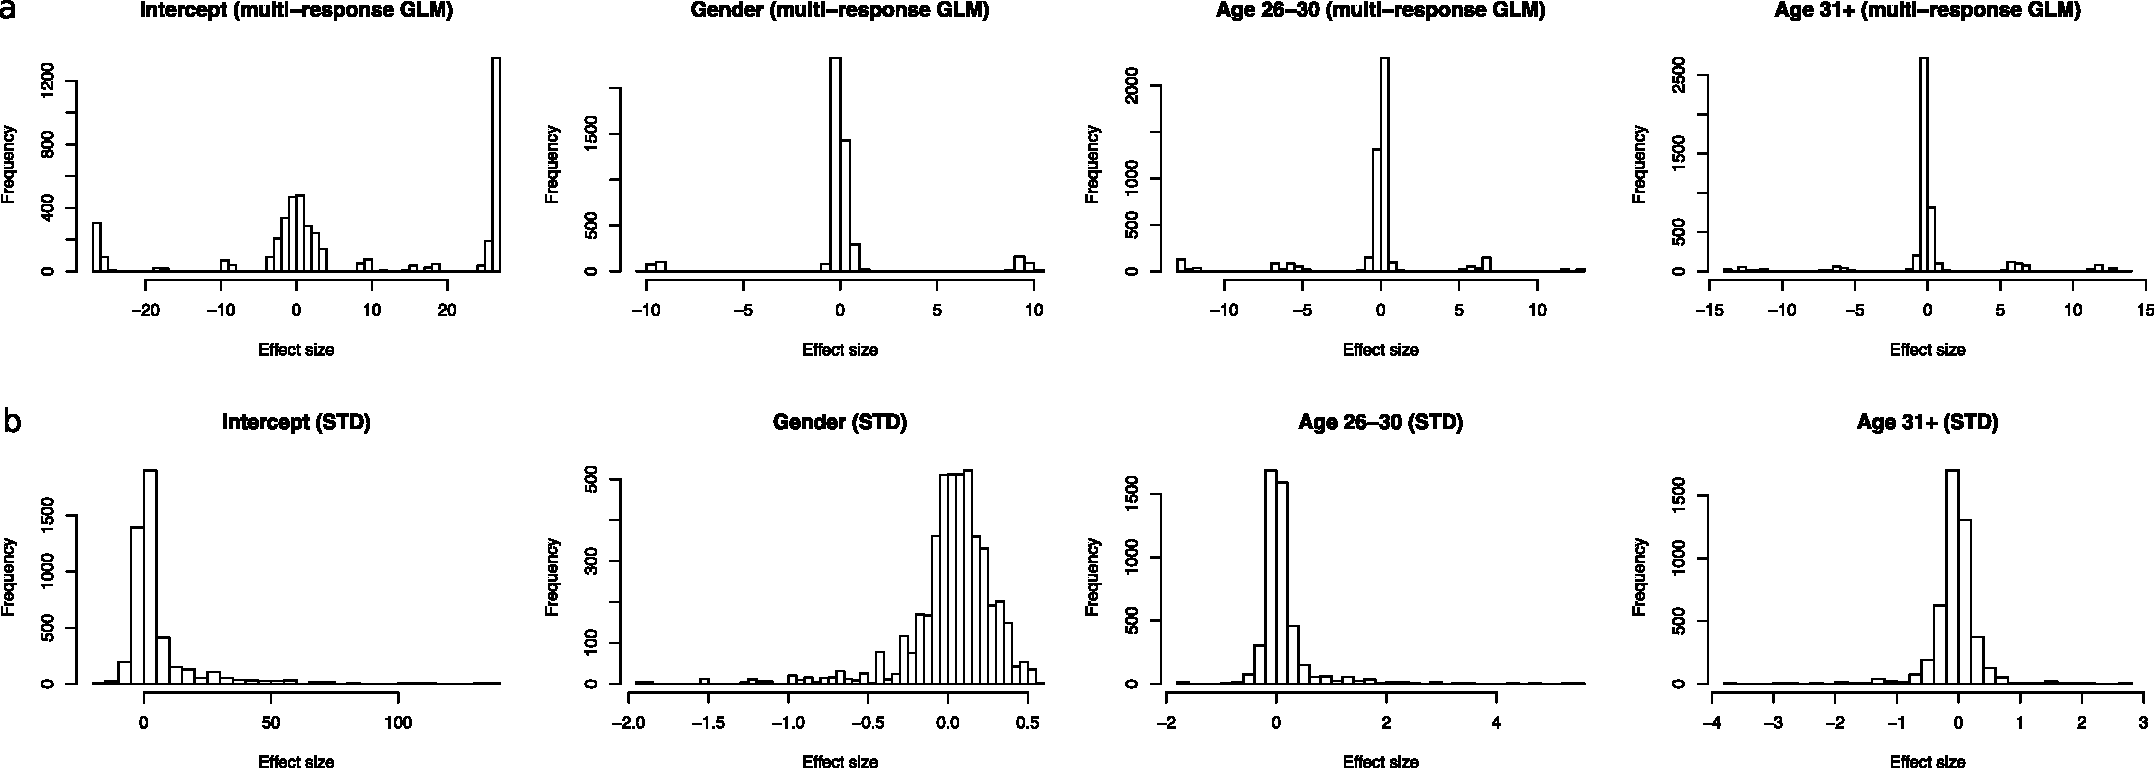
\includegraphics[width=14cm]{compare_HCP.pdf}
%\caption{Comparison of estimated feature effects the HCP data using (a) multi-response GLM and (b) supervised tensor decomposition (STD). }\label{fig:s1}
%\vspace{-.1cm}
\end{figure}


We perform the supervised tensor decomposition to the HCP data. %The data tensor is binary, $\tY\in\{0,1\}^{68\times 68\times 136}$, and the features are of dimension 4 on the 3$^{\text{rd}}$ mode. 
The BIC selection suggests a rank $\mr=(10,10,4)$ with quasi log-likelihood $\tL_{\tY}=-174654.7$. We utilize the sum-to-zero contrasts in coding the feature effects, and depict only the top 3\% edges whose connections are non-constant across the sample. Figure~\ref{fig:brain} shows the top edges with high effect size, overlaid on the Desikan atlas brain template~\citep{desikan2006automated}. We find that the global connection exhibits clear spatial separation, and that the nodes within each hemisphere are more densely connected with each other (Figure~\ref{fig:brain}a). In particular, the superior-temproal (\emph{SupT}), middle-temporal (\emph{MT}) and Insula are the top three popular nodes in the network. Interestingly, female brains display higher inter-hemispheric connectivity, especially in the frontal, parental and temporal lobes (Figure~\ref{fig:brain}b). This is in agreement with a recent study showing that female brains are optimized for inter-hemispheric communication~\citep{ingalhalikar2014sex}. We find several edges with declined connection in the group Age 31+. Those edges involve Frontal-pole (\emph{Fploe}), superior-frontal (\emph{SupF}) and Cuneus nodes. The Frontal-pole region is known for its importance in memory and cognition, and the detected decline with age further highlights its biological importance. 




\bibliography{tensor_wang}
\bibliographystyle{apalike}

\end{document}
